\documentclass[tikz,border=3pt]{standalone}
\usepackage[utf8]{inputenc}
\usepackage[T1]{fontenc}
\usepackage{lmodern}
\renewcommand{\familydefault}{\sfdefault}
\usepackage{sansmath}\sansmath
\usepackage{chemfig}
\usepackage{pgfplots}\pgfplotsset{compat=1.18,/pgf/number format/use comma,/pgf/number format/1000 sep={.}}
\usetikzlibrary{arrows.meta,calc,positioning,decorations.pathmorphing,patterns}
% paleta del sitio
\definecolor{nar}{HTML}{E8680C}\definecolor{narc}{HTML}{FFB35C}\definecolor{hielo}{HTML}{FFF3E8}
\definecolor{tinta}{HTML}{1D1D1F}\definecolor{gris}{HTML}{6E6E73}\definecolor{lila}{HTML}{7C5CF0}
\definecolor{azul}{HTML}{2F6FD6}\definecolor{menta}{HTML}{17A673}\definecolor{coral}{HTML}{E8342A}
\begin{document}
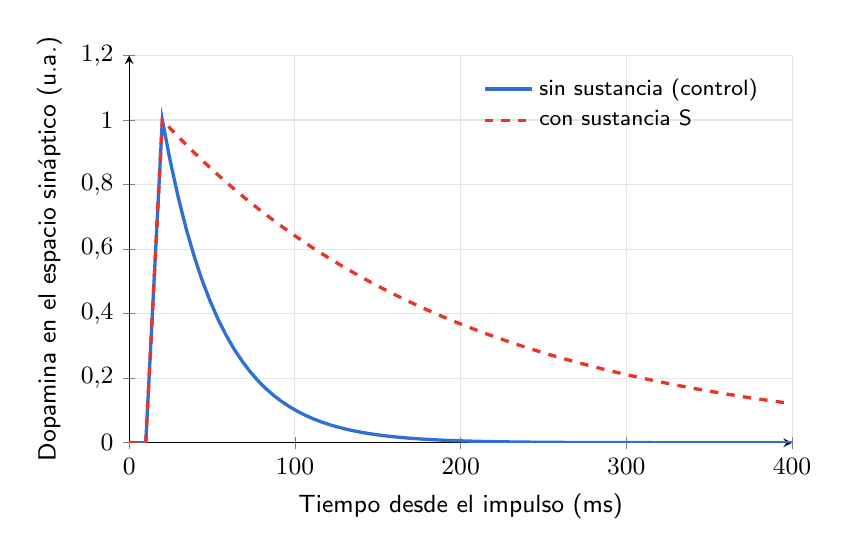
\begin{tikzpicture}[font=\small]
\begin{axis}[axis lines=left,grid=major,grid style={gray!20},xlabel={Tiempo desde el impulso (ms)},ylabel={Dopamina en el espacio sináptico (u.a.)},
  width=10cm,height=6.5cm,xmin=0,xmax=400,ymin=0,ymax=1.2,xtick={0,100,...,400},ytick={0,0.2,...,1.2},
  legend style={draw=none,fill=none,font=\footnotesize,at={(0.97,0.97)},anchor=north east},legend cell align=left]
\addplot[azul,very thick] coordinates {(0,0)(10,0)(20,1)} -- plot[domain=20:400,samples=80] ({\x},{exp(-(\x-20)/35)});
\addlegendentry{sin sustancia (control)}
\addplot[coral,very thick,dashed] coordinates {(0,0)(10,0)(20,1)} -- plot[domain=20:400,samples=80] ({\x},{exp(-(\x-20)/180)});
\addlegendentry{con sustancia S}
\end{axis}
\end{tikzpicture}
\end{document}
